\documentclass{beamer}
\usepackage[utf8]{inputenc}
\usepackage[newfloat]{minted}
\usepackage{caption}

\newenvironment{code}{\captionsetup{type=listing}}{}
\SetupFloatingEnvironment{listing}{name=Source Code}


\usepackage{utopia} %font utopia imported

\usetheme{Goettingen}
\usecolortheme{default}

\def\vfilll{\vskip 0pt plus 1filll minus 0pt }

\title{Initiation au développement informatique}
\author{Matthieu Falce \& Jordan Bouchoucha}

\institute{Association des Bidouilleurs Libristes}

\date{Novembre 2017}

\begin{document}

    \vfilll
    \titlepage
    \vfilll
    \usebeamerfont{institute} Contact : \linebreak 
    	\phantom{pasvu} $\circ$ \url{matthieu@falce.net} \linebreak 
    	\phantom{pasvu} $\circ$ \url{jordan.bouchouch@gmail.com}


    \title{Faire une page web interactive de A à Z à travers un petit jeu }
    \begin{frame}
    \maketitle
    \end{frame}

    \title{Faire une page web interactive de A à Z à travers un petit jeu \linebreak \small{tout nul et tout moche}}
    \begin{frame}
    \maketitle
    \end{frame}
    
    \title{Initiation au développement informatique}

   \begin{frame}
        \frametitle{Au programme}
        \tableofcontents
   \end{frame}

    \section{Préparation}

    \begin{frame}
		\frametitle{Ca ne sera pas facile}
		\centering 
\includegraphics[width=10cm]{images/goals_imagination_reality.png} 
    \end{frame}

    \begin{frame}
		\frametitle{Mais ça en vaut la peine}
		\centering 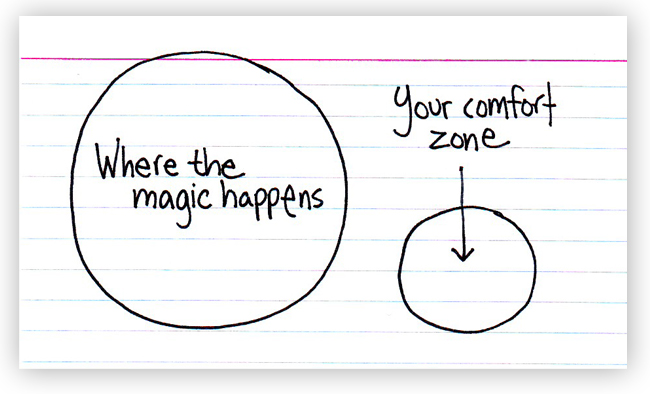
\includegraphics[width=10cm]{images/wherethemagichappens.jpg} 
    \end{frame}

    \subsection{Editeur de texte}
    \begin{frame}
		\frametitle{Editeur de texte}

    	Utiliser un bon éditeur de texte est primordial.
        \begin{itemize}
			\item{Télécharger et installer \url{https://www.sublimetext.com/3}}
			\item{Installer le plugin Emmet (ctrl/cmd-maj-p puis install package)}	
        \end{itemize}
		
    \end{frame}

    \subsection{Fichiers}
    \begin{frame}
		\frametitle{Fichiers}

        Créer deux fichiers
        \begin{itemize}
          \item code.js : pour vos tests
          \item index.html : pour le vrai code du site
        \end{itemize}
        
        \vspace{1cm}
        \centering Vous pouvez glisser les fichiers html dans votre navigateur pour les interpréter.
    \end{frame}

    \section{Javascript}
    \begin{frame}
		\frametitle{Javascript}
		\centering 
\includegraphics[width=4cm]{images/js.jpg} 
    \end{frame}

    \begin{frame}
		\frametitle{Javascript}
		\centering 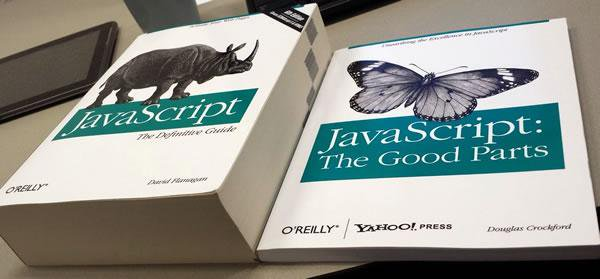
\includegraphics[width=10cm]{images/complete_javascript_vs_good_parts.jpeg} 
    \end{frame}

    \begin{frame}
		\frametitle{Javascript ?}
		\begin{itemize}
			\item Langage de développement pour navigateurs
			\item concepts de base : 
				\begin{itemize}
					\item variable (et leur types)
					\item fonction
					\item méthodes de comparaison
					\item boucle
				\end{itemize}
		\end{itemize}
    \end{frame}

    \subsection{Bases}
    \begin{frame}
		\frametitle{Bases}

		\begin{center}
			Bientôt, vos premières lignes de code.
		\end{center}		 
	
		\vspace{1cm}

		Modifier le fichier code.js
        \begin{itemize}
          \item{utiliser sublime text}
          \item{copier / coller le code dans la console JS d'un navigateur}
        \end{itemize}

		\vspace{1cm}

		\centering Développement web $\Rightarrow$ vous avez tous les outils 
    \end{frame}

	\subsection{Live Coding -- brainstorming}
	\begin{frame}
		\frametitle{Live Coding -- brainstorming}
	\end{frame}

	\subsection{Au boulot !}
    \begin{frame}
		\frametitle{C'est à vous}
		\centering Codez le jeu permettant de faire deviner un nombre à l'utilisateur.
    \end{frame}

	\section{HTML}
	\begin{frame}
		\frametitle{HTML5}
		\centering 
\includegraphics[width=5cm]{images/HTML5_Logo_512.png} 
    \end{frame}
    
	\subsection{Bases}
	\begin{frame}
		\frametitle{HTML ?}
		\begin{itemize}
			\item Langage de description des pages internet
			\item Imbriquer des rectangles dans d'autres rectangles
            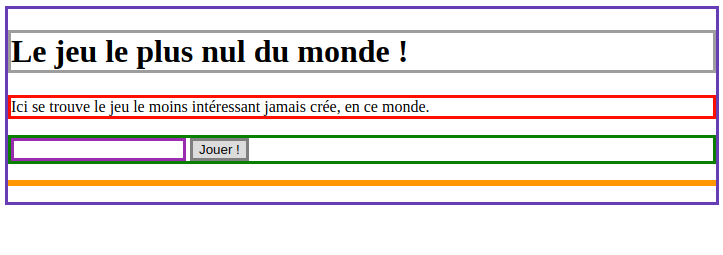
\includegraphics[width=5cm]{images/html_structure.png}
			\item concepts de base : 
				\begin{itemize}
					\item body
					\item titre (h1, h2, h3)
					\item conteneurs (div, p...)
					\item UI (input, bouton)
				\end{itemize}
		\end{itemize}
    \end{frame}

	\subsection{Représentation}

	\begin{frame}[fragile]
		\frametitle{Représentation -- code}

		\begin{figure}
			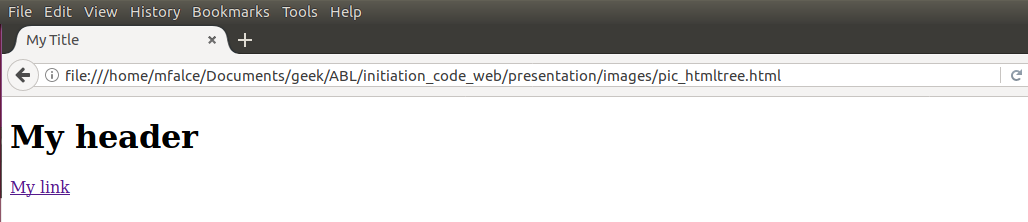
\includegraphics[width=8cm]{images/page_html.png}
			\caption{page web basique}	
		\end{figure}
		
		\begin{code}
			\inputminted{html}{images/pic_htmltree.html}
			\captionof{listing}{Code HTML de la page ci-dessus}
		\end{code}				
		
	\end{frame}		

	\begin{frame}
		\frametitle{Représentation -- Boites}

		\begin{figure}
			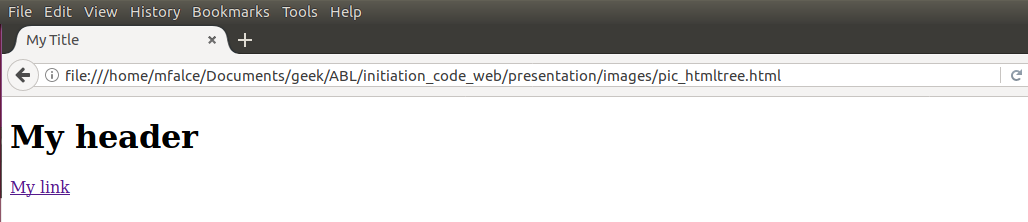
\includegraphics[width=8cm]{images/page_html.png}
			\caption{Page web basique}	
		\end{figure}
		
		\begin{figure}
			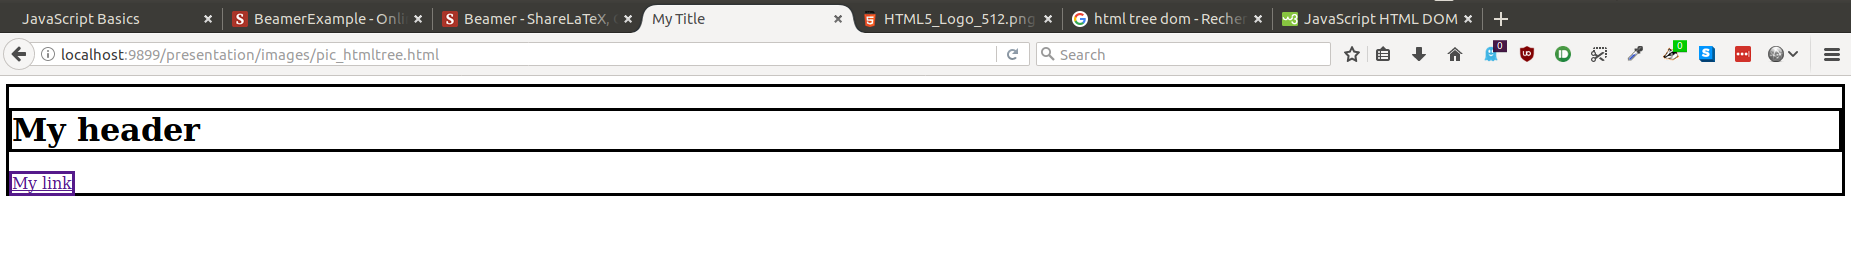
\includegraphics[width=10cm]{images/pic_htmltree_resultat.png}
			\caption{Boites avec leurs éléments}	
		\end{figure}		
		
	\end{frame}	

	\begin{frame}
		\frametitle{Représentation -- Arbre}

		\begin{figure}
			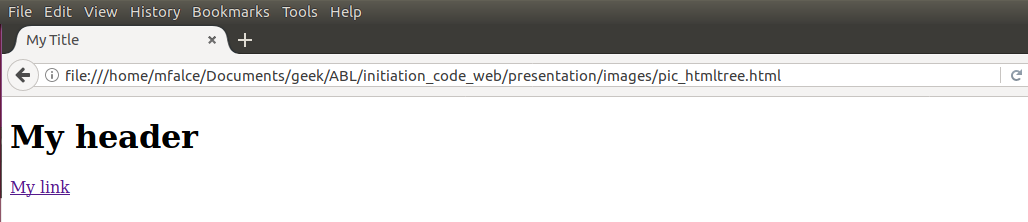
\includegraphics[width=8cm]{images/page_html.png}
			\caption{Page web basique}	
		\end{figure}
		
		\begin{figure}
			\includegraphics<1>[width=8cm]{images/pic_htmltree_dom_1.png}
			\includegraphics<2>[width=8cm]{images/pic_htmltree_dom_2.png}
			\includegraphics<3>[width=8cm]{images/pic_htmltree_dom_3.png}
			\includegraphics<4>[width=8cm]{images/pic_htmltree_dom_4.png}
			\includegraphics<5>[width=8cm]{images/pic_htmltree_dom_5.png}
			\includegraphics<6>[width=8cm]{images/pic_htmltree_dom_6.png}
			\includegraphics<7>[width=8cm]{images/pic_htmltree_dom_7.png}
			\includegraphics<8>[width=8cm]{images/pic_htmltree_dom_8.png}
			\includegraphics<9>[width=8cm]{images/pic_htmltree_dom_9.png}
			\includegraphics<10>[width=8cm]{images/pic_htmltree_dom_10.png}
			\caption{Arbre du document}	
		\end{figure}		
		
	\end{frame}	
	
	\begin{frame}
		\frametitle{Représentation -- Arbre -- Pour info}

		\begin{figure}
			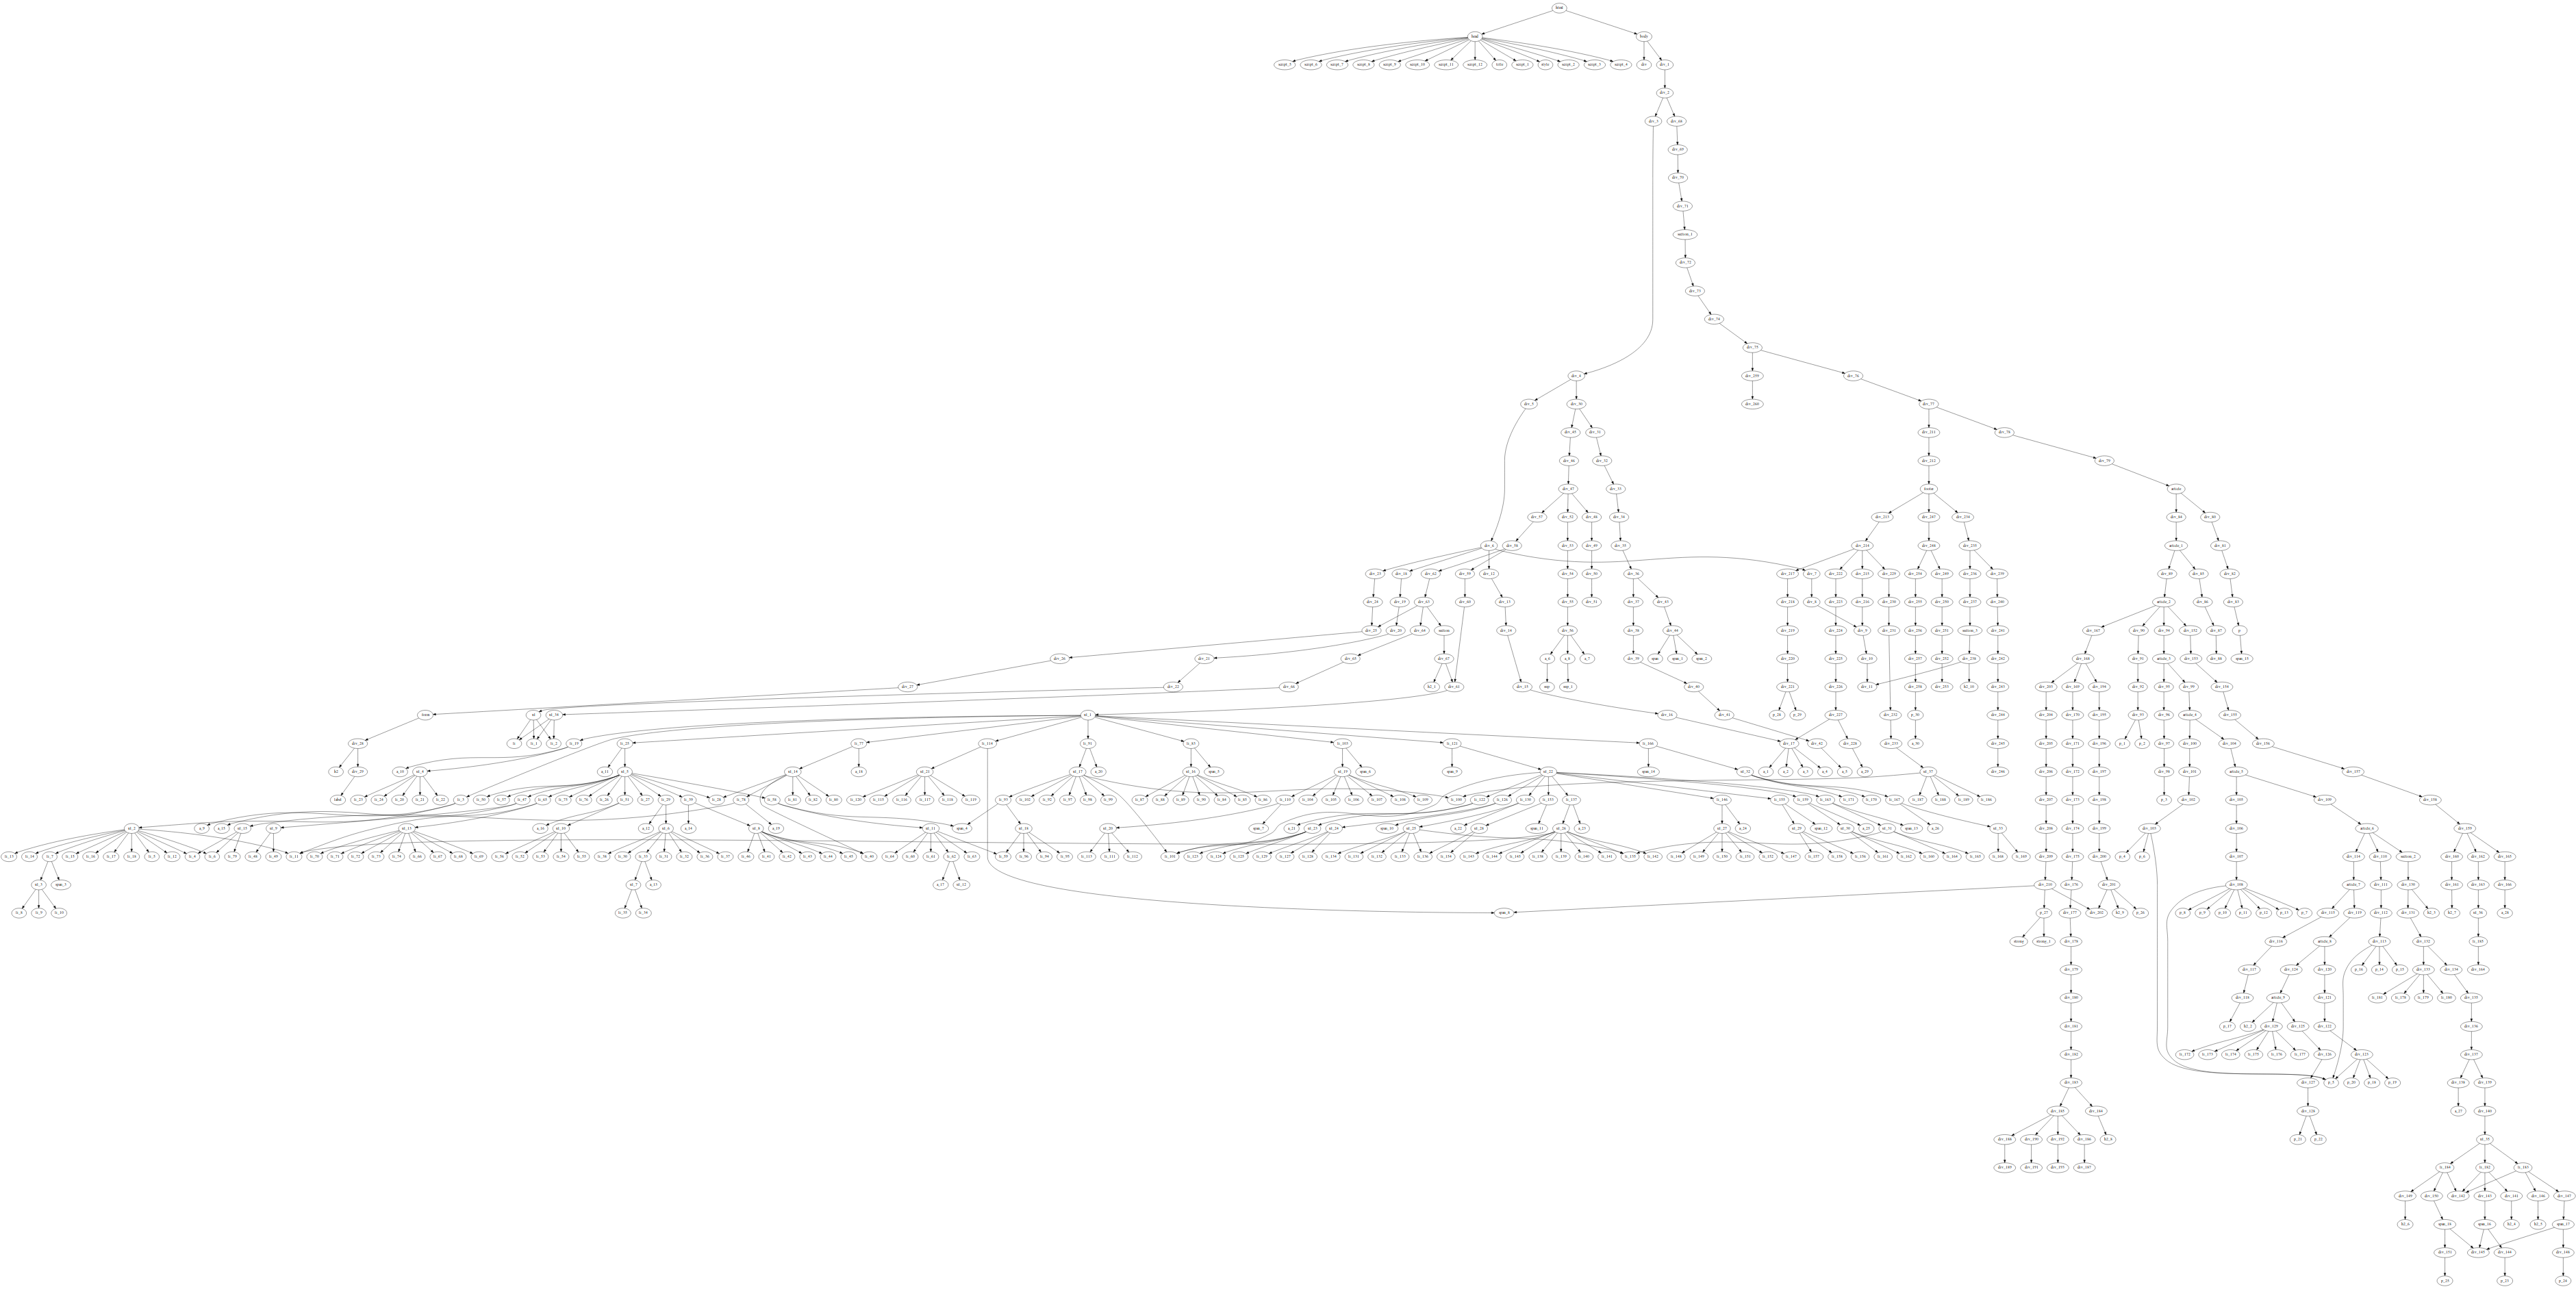
\includegraphics[width=10cm]{images/page_acceuil_sciences_po_dom.png}
			\caption{\url{http://www.sciencespo-lille.eu/}}	
		\end{figure}		
		
	\end{frame}	
	
	
	
	
	\subsection{Live Coding}
	\begin{frame}
		\frametitle{C'est à nous}
	\end{frame}

	
	\subsection{Au boulot !}
	\begin{frame}
		\frametitle{C'est à vous}
		Codez la page avec : 
		\begin{itemize}
			\item une structure HTML classique (Head, Body, ...)
			\item un titre expliquant la page
			\item un paragraphe avec les règles du jeu
			\item une zone de jeu
				\begin{itemize}
					\item une zone pour entrer du texte
					\item un bouton pour valider
					\item un paragraphe donnant une indication à l'utilisateur
				\end{itemize}
		\end{itemize}
	\end{frame}

	\section{CSS}
	\begin{frame}
		\frametitle{CSS}
		\centering 
\includegraphics[width=5cm]{images/css3.png} 
    \end{frame}
	
	\subsection{Bases}
    \begin{frame}
    	\frametitle{CSS?}
		\begin{itemize}
			\item Cascading Style Sheet
			\item Modifie le style visuel d'une page HTML
			\item Séparation contenu -- style
			\item concepts de base : 
				\begin{itemize}
					\item sélecteurs
					\item relation entre les sélecteurs
				\end{itemize}
		\end{itemize}

		\vspace{1cm}
		\centering Sélection d'élément $\Rightarrow$ arbre HTML		
		
    \end{frame}
	
	\subsection{Live Coding}
	    \begin{frame}
    	\frametitle{C'est à nous}
		\centering Améliorons le site \emph{le plus moche du monde}. \url{http://www.goldnuggetwebs.com/worstweb-fr/index.html}
    \end{frame}
	
	\subsection{Au boulot !}
	\begin{frame}
		\frametitle{C'est à vous}
		Rendez votre jeu plus agréable à l’œil :
		\begin{itemize}
			\item Changez les couleurs de textes
			\item Changez les couleurs de fond selon la réponse donnée
			\item Centrez les éléments
			\item ...
		\end{itemize}
	\end{frame}

	\section{Conclusion}
	\begin{frame}
		\frametitle{Pour conclure}
		\begin{itemize}
			\item Apprendre en faisant
			\item Le but n'est pas de tout comprendre
			\item Aborder la logique à avoir
			\item Comprendre le vocabulaire
			\item \emph{Magic's gone :)}
		\end{itemize}
	\end{frame}
	
	\subsection{Ouverture}
	\begin{frame}
		\frametitle{Aller plus loin}
		Des ressources en vrac pour s'améliorer. 

		\vspace{0.4cm}
		Généraux : 
		\begin{itemize}
			\item Support du cours : \url{https://github.com/bidouilleurslibristes/initiation_code_web} 
			\item la bible du développeur web : \url{https://developer.mozilla.org/}
		\end{itemize}	
		
		\vspace{0.4cm}
		Cours en ligne : 
		\begin{itemize}
			\item Cours en ligne HTML / JS / CSS (en anglais) : \url{https://www.udacity.com/course/html-and-css-syntax--ud001}
			\item The Coding Train (chaine youtube en anglais, orienté "oeuvres d'art / contenu intéractif") : \url{https://www.youtube.com/channel/UCvjgXvBlbQiydffZU7m1_aw}
		\end{itemize}			
		
		\vspace{0.4cm}		
		Articles divers : 
		\begin{itemize}
			\item https://autotelicum.github.io/Smooth-CoffeeScript/literate/js-intro.html
			\item \url{https://developer.mozilla.org/en-US/docs/Learn/CSS/Introduction_to_CSS/Simple_selectors}
			\item \url{http://www.cssbasics.com}
		\end{itemize}
	\end{frame}
	
\end{document}



